\section{Экзамен}

\subsection{Базы данных и системы управления базами данных. Определения, основные функции и классификация}

\textbf{База данных} (БД) ---  самодокументированное собрание интегрированных записей.

\begin{enumerate}
	\item БД является самодокументированной, т.е. она содержит описание собственной структуры. Это описание называется словарем данных, каталогом данных или метаданными.
	\item БД является собранием интегрированных записей, т.е. она содержит:
	\begin{itemize}
		\item файлы данных;
		\item метаданные (данные о данных);
		\item индексы, которые представляют связи между данными, а также служат для повышения производительности приложений базы данных;
		\item метаданные приложения.
	\end{itemize}
	\item БД является информационной моделью пользовательской модели предметной области.
\end{enumerate}

\textbf{OLAP} --- online analtyc proccesing (операциооные данные).

\textbf{OLTP} --- online transaction proccessing (перманентые данные).

\begin{table}[ht!]
	\begin{center}
		\caption{}
		\label{tbl:best}
		\begin{tabular}{|c|c|}
			\hline
			OLAP & OLTP \\
			\hline
			чтение & вставка, удаление, обновление \\
			\hline
			минимальное время отклика & минимальное время вставки, удаление, обновление \\
			\hline
		\end{tabular}
	\end{center}
\end{table}

\textbf{Транзакции} --- либо все действия, либо никакие действия.


\textbf{Любая бд хранит}:

\begin{enumerate}
	\item метаданные (данные о данных);
	\item файлы данных,
	\item Индексы (indexes), которые представляют связи между данными,  a также служат для повышения производительности приложений базы данных.
	\item Может содержать метаданные приложений (application metadata).
\end{enumerate}

\textbf{Основные храктеристики, требования}

\begin{enumerate}
	\item \textbf{Неизбыточность данных} --- каждое данное присутствует в БД в единственном экземпляре.
	\item \textbf{Совместное использование данных} многими пользователями.
	\item \textbf{Эффективность доступа} к БД - высокое быстродействие, т. е. малое время отклика на запрос.
	\item \textbf{Целостность данных} --- соответствие имеющейся в БД информации её внутренней логике, структуре и всем явно заданным правилам.
	\item \textbf{Безопасность данных} --- защита данных от преднамеренного или непреднамеренного искажения или разрушения данных.
	\item \textbf{Восстановление данных} после программных и аппаратных сбоев.
	\item \textbf{Независимость данных} от прикладных программ.
\end{enumerate}

\textbf{Система баз данных} (СБД) --- совокупность одной или нескольких баз данных и комплекса информационных, программных и технических средств, обеспечивающих накопление, обновление, корректировку и многоаспектное использование данных в интересах пользователей.

\textit{Система управления базами данных} (СУБД) --- приложение, обеспечивающее создание, хранение, обновление и поиск информации в базах данных.

\textbf{Основные функции СУБД}

\begin{enumerate}
	\item Управление данными во внешней памяти.
	\item Управление буферами оперативной памяти.
	\item Управление транзакциями.
	\item Журнализация.
	\item Поддержка языка или языкового пакета (-ов).
\end{enumerate}

\textbf{Классификация СУБД}:
\begin{enumerate}
	\item По модели данных:
	\begin{itemize}
		\item Дореляционные (Инвертированные списки, иерархические и сетевые)
		\begin{itemize}
			\item Инвертированные списки (файлы). БД на основе инвертированных списков представляет собой совокупность файлов, содержащих записи (таблиц). Для записей в файле определен некоторый порядок, диктуемый физической организацией данных. Для каждого файла может быть определено произвольное число других упорядочений на основании значений некоторых полей записей (инвертированных списков). Обычно для этого используются индексы. В такой модели данных отсутствуют ограничения целостности как таковые. Все ограничения на возможные экземпляры БД задаются теми программами, которые работают с БД. Одно из немногих ограничений, которое все-таки может присутствовать - это ограничение, задаваемое уникальным индексом. 
			\item Иерархичекие
			\item Сетевые (могут быть представлены в виде графа; логика выборки зависит от физической организации данных)
		\end{itemize}
		\item Реляционные
		\begin{itemize}
			\item Структурный (данные --- набор отношений)
			\item Целостностный (отношения (таблицы) отвечают определенным условиям целостности)
			\item Манипуляционный (манипулирования отношениями осуществляется средствами реляционной алгебры и/или реляционного исчисления)
		\end{itemize}
		\item Постреляционные
	\end{itemize}
	\item По архитектуре организации хранения данных:
	\begin{itemize}
		\item Локальные (все части локальной СУБД размещаются на одном компьютере)
		\item Распределенные (части СУБД могут размещаться на 2-х и более компьютерах) 
	\end{itemize}
	\item По способу доступа к БД:
	\begin{itemize}
		\item Файл-серверные (при работе с базой, данные перегоняются приложению, которое с ней работает, вне зависимости от того, сколько их нужно. Все операции --- на стороне клиента. Файловый сервер периодически обновляется тем же клиентом)
		\item Клиент-серверные (вся работа на сервере, по сети передаются результаты запросов, гораздо меньше информации. Обеспечивается безопасность данных, потому что все происходит на стороне сервера. Проще исключить одновременное изменение и тп)
		\item Встраиваемые --- библиотека, которая позволяет унифицированным образом хранить 
		большие объемы данных на локальной машине. Доступ к данным может происходить через SQL либо через 
		особые функции СУБД. Встраиваемые СУБД быстрее обычных клиент-серверных и не требуют установки 
		сервера, поэтому востребованы в локальном ПО, которое имеет дело с большими объемами данных.
		\item Сервисно-ориентированные  (БД является хранилищем сообщений, промежуточных состояний, метаинформации об очередях сообщений и сервисах)
		\item Прочие (пространственная, временная и пространственно-временная)
	\end{itemize}
\end{enumerate}

\textbf{Архитектура хранения данных}

\begin{enumerate}
	\item Локальные.
	\item Распределенные.
	\item По способу обращения к данным.
	\begin{itemize}
		\item Файл серверные.
		\item Клиент серверные (PostGress, MSSQL, Oracle, MySQL, Mongo).
		\item Встраиваемые (SQLlite).
		\item Сервисно-ориентированные (KafcaBD).
		\item Прочее - time series.
	\end{itemize}
\end{enumerate}

\subsection{Семантическое моделирование данных}

Любая развитая семантическая модель данных, как и реляционная модель, включает структурную, манипуляционную и целостную части. Главным назначением семантических моделей является обеспечение возможности выражения семантики данных. На практике семантическое моделирование используется на первой стадии проектирования базы данных. При этом в терминах семантической модели производится концептуальная схема базы данных, которая затем:
\begin{enumerate}
	\item Либо вручную преобразуется к реляционной схеме;
	\item Либо реализуется автоматизированная компиляция концептуальной схемы в реляционную;
	\item Либо происходит работа с базой данных в семантической модели, т.е. под управлением СУБД, основанных на семантических моделях данных. 
\end{enumerate}

Наиболее известным представителем класса семантических моделей предметной области является модель «сущность-связь» или ER-модель, , предложенная Питером Ченом в 1976 году.

Модель сущность-связь — модель данных, позволяющая описывать концептуальные схемы предметной области. Предметная область — часть реального мира, рассматриваемая в пределах данного контекста. Под контекстом здесь может пониматься, например, область исследования или область, которая является объектом некоторой деятельности. ER-модель используется при высокоуровневом (концептуальном) проектировании баз данных.

Основными понятиями ER-модели являются сущность, связь и атрибут(свойство).

Сущность - это реальный или представляемый объект, информация о котором должна сохраняться и быть доступна. При этом имя сущности - имя типа, а не некоторого конкретного экземпляра этого типа. Каждый экземпляр сущности должен быть отличим от любого другого экземпляра этой сущности.

Связь - это ассоциация, устанавливаемая между сущностями. Эта ассоциация может существовать между разными сущностями или между сущностью и ей же самой (рекурсивная связь). Сущности, включенные в связь, называются её участниками, а количество участников - степенью связи. Связи в ER-модели могут иметь тип <<один к одному>>, <<один ко многим>>, <<многие ко многим>>.

Свойством/атрибут сущности (и связи) является любая деталь, которая служит для уточнения, идентификации, классификации, числовой характеристики или выражения состояния сущности (или связи).

Ключи: Первичный ключ --- набор атрибутов однозначно идентифицирующий кортеж значений, и Внешний ключ

\subsection{Реляционная модель данных: структурная, целостная, манипуляционная части. Реляционная алгебра. Исчисление кортежей}

Реляционная модель данных согласно трактовке Кристофера Дейта состоит из трех частей: структурной, целостной и манипуляционной.

\textbf{Структурная часть} описывает из каких объектов состоит реляционная модель. Основной структурой данных в реляционной модели является нормализованные n-мерные отношения и основными понятиями структурной части реляционной модели является:
\begin{itemize}
	\item \textit{Тип данных} --- множество значений и операций над ними. (понятие такое же как и в языках программирования);
	\item \textit{Домен} можно считать уточнением типа данных и рассматривать как подмножество значений некоторого типа данных, имеющий определенный смысл. 
	Характеризуется следующими свойствами:
	\begin{itemize}
		\item имеет уникальное имя в пределах базы данных;
		\item определен на некотором типе данных или на другом домене;
		\item может иметь логическое условие, позволяющее описать подмножество данных, доступных для данного домена;
		\item несет определенную смысловую нагрузку
	\end{itemize}
	Домен отражает семантику, определенной предметной области и может быть не сколько доменов совпадающих как подмножество, но с различным смыслом. Основное значения домена ограничивается сравнением.
	\item \textit{Атрибут отношения} --- это пара вида <имя\_атрибута, имя\_домена>, при этом имена атрибутов должны быть уникальны в пределах отношения, но могут совпадать с именем домена.
	\item \textit{Схема отношения} --- это именованное множество упорядоченных пар <имя\_атрибута, имя\_домена>.
	\item \textit{Схема БД} --- это множество именованных схем отношений.
	\item \textit{Кортеж} --- это множество упорядоченных пар <имя\_атрибута, значение\_атрибута>, которое содержит одно вхождение каждого имени атрибута, принадлежащего схеме отношения.
	\item \textit{Отношение} определенное на множестве из n доменов (не обязательно различных), содержит две части: заголовок (схему отношения) и тело (множество из m кортежей). Значения n и m называются соответственно степенью и кардинальностью отношения.
	\item Непустое подмножество множества атрибутов схемы отношения будет \textit{потенциальным ключом} тогда и только тогда, 
	когда оно будет обладать свойствами уникальности (в отношении нет двух различных кортежей с одинаковыми 
	значениями потенциального ключа) и неизбыточности (никакое из собственных подмножеств множества 
	потенциального ключа не обладает свойством уникальности). 
	\item В реляционной модели по традиции один из потенциальных ключей должен быть выбран в качестве \textit{первичного ключа}, а все остальные потенциальные ключи будут называться \textit{альтернативными}.
	\item \textit{Реляционная база данных} --- это набор отношений, имена которых совпадают с именами схем отношений в схеме базы данных.
\end{itemize}

\textbf{Целостностная часть} описывает ограничения специального вида, которые должны выполняться для любых отношений в любых реляционных базах данных. Это целостность сущностей и целостность внешних ключей.

\textbf{Манипуляционная часть} описывает два эквивалентных способа манипулирования реляционными данными - реляционную алгебру и реляционное исчисление.

\textbf{Реляционная алгебра} является основным компонентом реляционной модели, опубликованной Коддом, и состоит из восьми операторов, составляющих две группы по четыре оператора:
\begin{itemize}
	\item Традиционные операции над множествами: объединение (UNION), пересечение (INTERSECT), разность (MINUS) и декартово произведение (TIMES). Все операции модифицированы, с учетом того, что их операндами являются отношения, а не произвольные множества.
	\item Специальные реляционные операции: ограничение (WHERE) , проекция (PROJECT), соединение (JOIN) и деление (DIVIDE BY).
\end{itemize}

Результат выполнения любой операции реляционной алгебры над отношениями также является отношением. Эта особенность называется свойством реляционной замкнутости. Утверждается, что поскольку реляционная алгебра является замкнутой, то в реляционных выражениях можно использовать вложенные выражения сколь угодно сложной структуры.

\textbf{Исчисление} существует в двух формах: исчисление кортежей и исчисление доменов. Основное различие между ними состоит в том, что переменные исчисления кортежей являются переменными кортежей (они изменяются на отношении, а их значения являются кортежами), в то время как переменные исчисления доменов являются переменными доменов (они изменяются на доменах, а их значения являются скалярами).

Выражение исчисления кортежей содержит заключенный в скобки список целевых элементов и выражение WНERE, содержащее формулу WFF ("правильно построенную формулу"). Такая формула WFF составляется из кванторов (EXISTS и FORALL), свободных и связанных переменных, литералов, операторов сравнения, логических (булевых) операторов и скобок. Каждая свободная переменная, которая встречается в формуле WFF, должна быть также перечислена в списке целевых элементов.

\subsection{Теория проектирования реляционных баз данных: функциональные зависимости, нормальные формы}

Пусть 


\subsection{Теория проектирования хранилищ данных. Основные принципы построения. ETL и ELT процессы}

\textbf{Определение}

\subsection{Транзакции. Определение, свойства и уровни изоляции транзакций. Неблагоприятные эффекты, вызванные параллельным выполнением транзакци , и способы их устранения. Управление транзакциями и способы обработки ошибок}

\textbf{Свойства} для n = 2


\subsection{Блокировки. Определение, свойства, иерархии, гранулярность и взаимоблокировки, алгоритмы обнаружения взаимоблокировок}

\textbf{Определение}

Блокировка --- это механизм, с помощью которого компонент Database Engine
синхронизирует одновременный доступ нескольких пользователей к одному фрагменту данных.

\textbf{Свойства}

\begin{enumerate}
	\item гранулярностью (или размером блокировки)
	\item режимом (или типом блокировки)
	\item продолжительностью
\end{enumerate}

\textbf{Гранулярность}




\subsection{Журнализация. Операции журнала транзакций и его логическая и физическая архитектуры. Модели восстановления. Метаданные}

\textbf{Нет вопроса}

\subsection{Безопасность и Аудит. Ключевые понятия и участники системы безопасности. Модели управления доступом}

\textbf{Этого вопроса нет}


\subsection{MPP системы. Распределенное и колоночное хранение. Распределенные вычисления, модель MapReduce. Обеспечение отказоустойчивости.}

Пусть

\subsection{In-Memory базы данных. Преимущества и недостатки. Примеры использования}

Учитывая равенство $P\{Y < y\} = 	F_Y(y)$, приходим к формуле \ref{jopa2}.

\subsection{Инструкции языка описания данных, инструкции языка обработки данных, инструкции безопасности, инструкции управления транзакциями}

Когда $X_1, X_2$ являются \textit{независимыми случайными величинами, то есть их двумерная плотность распределения}



\subsection{Объекты базы данных: функции, процедуры, триггеры и курсоры}


\subsection{Оптимизация запроса: индексы, партиционирование, сегментирование}

\subsubsection{Индексы}
\textit{(материал на основе SQL Server)}

Индекс – это объект базы данных, обеспечивающий дополнительные способы быстрого поиска и извлечения данных. Индекс может создаваться на одном или нескольких столбцах. 
Это означает, что индексы бывают простыми и составными. Если в таблице нет индекса, то поиск нужных строк выполняется простым сканированием по всей таблице. При наличии индекса время поиска нужных строк можно существенно уменьшить. 

К недостаткам индексов следует отнести:
\begin{itemize}
	\item дополнительное место на диске и в оперативной памяти, 
	\item замедляются операции вставки, обновления и удаления записей. 
\end{itemize}

В SQL Server (и, наверное, многих других СУБД) индексы хранятся в виде сбалансированных деревьев. Представление индекса в виде сбалансированного дерева означает, что стоимость поиска любой строки остается относительно постоянной, независимо от того, где находится эта строка. 

\begin{figure}[h]
	\centering
	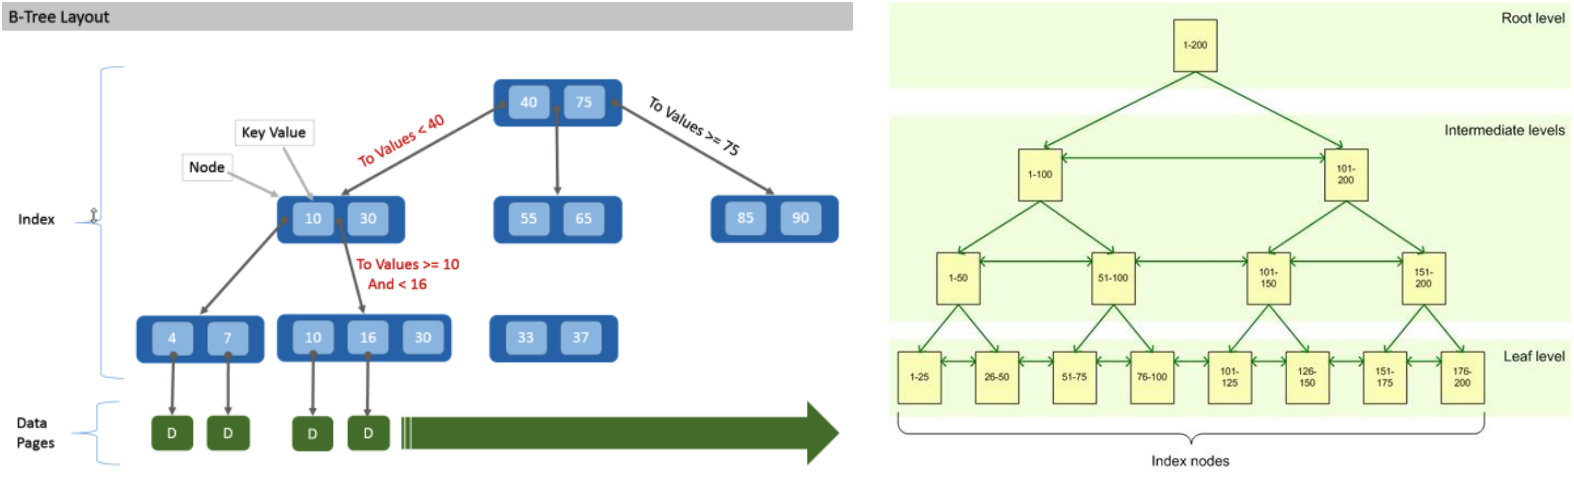
\includegraphics[width=18cm, keepaspectratio]{assets/index.png}
	\caption{B-Tree} 
\end{figure}

Существует два типа индексов: 

\begin{itemize}
	\item Кластерные индексы
	\item Некластерные индексы, которые включают: 
	\begin{itemize}[label=--]
		\item индексы на основе кучи;
		\item индексы на основе кластерных таблиц.
	\end{itemize}
\end{itemize}

\textbf{Кластерные индексы}

В кластерном индексе таблица представляет собой часть индекса, или индекс представляет собой часть таблицы в зависимости от вашей точки зрения. Листовой узел кластерного индекса – это страница таблицы с данными. Поскольку сами данные таблицы являются частью индекса, для таблицы может быть создан только один кластерный индекс. Кластерный индекс является уникальным индексом по определению.

\textbf{Некластерные индексы на основе кучи}

В листьях некластерного индекса на основе кучи хранятся указатели на строки данных. Указатель строится на основе идентификатора файла (ID), номера страницы и номера строки на странице. Весь указатель целиком называется идентификатором строки (RID).

\textbf{Некластерные индексы, основанные на кластерных таблицах}

В листьях некластерного индекса, основанного на кластерных таблицах, хранятся указатели на корневые узлы кластерных индексов. Поиск в таком индексе состоит из двух этапов:

\begin{itemize}
	\item поиск в некластерном индексе;
	\item поиск в кластерном индексе.
\end{itemize}

\textbf{Создание индекса}

В SQL Server индексы создаются при помощи команды \textbf{CREATE INDEX}.

Помимо этого, индексы создаются при добавлении некоторых ограничений. Такой тип индексов часто называют <<связанными индексами>>. Связанные индексы создаются при добавлении одного из следующих двух типов ограничений: 
\begin{itemize}
	\item ограничения первичного ключа (PRIMARY KEY); 
	\item ограничения уникальности (UNIQUE). 
\end{itemize}

\subsubsection{Партиционирование}
\textit{(материал на основе PostgreSQL)}

Партиционирование – это метод разделения больших (исходя из количества записей, а не столбцов) таблиц на много маленьких.

Для произведения партиционирования нужно решить, каким будет ключ партиционирования – другими словами, по какому алгоритму будут выбираться партиции. Есть пара наиболее очевидных: 
\begin{enumerate}
	\item партиционирование по дате – например, выбирать партиции, основываясь на годе, в котором пользователь был создан.
	
	\textit{Достоинства:}
	\begin{itemize}[label=--]
		\item легко понять;
		\item количество строк в данной таблице будет достаточно стабильным.
	\end{itemize}
	
	\textit{Недостатки:}
	\begin{itemize}[label=--]
		\item требует поддержки – время от времени нам придётся добавлять новые партиции;
		\item поиск по имени пользователя или id потребует сканирования всех партиций;
	\end{itemize}
	
	\item партиционирование по диапазону идентификаторов – например, первый миллион пользователей, второй миллион пользователей, и так далее
	
	\textit{Достоинства:}
	\begin{itemize}[label=--]
		\item легко понять;
		\item количество строк в данной таблице будет абсолютно стабильным.
	\end{itemize}
	
	\textit{Недостатки:}
	\begin{itemize}[label=--]
		\item требует поддержки – время от времени нам придётся добавлять новые партиции;
		\item поиск по имени пользователя потребует сканирования всех партиций; 
	\end{itemize}
	
	\item партиционирование по чему-нибудь другому – например, по первой букве имени пользователя. 
	
	\textit{Достоинства:}
	\begin{itemize}[label=--]
		\item легко понять;
		\item никакой поддержки --- есть строго определенный набор партиций и нам никогда не придется добавлять новые;
	\end{itemize}
	
	\textit{Недостатки:}
	\begin{itemize}[label=--]
		\item количество строк в партициях будет стабильно расти; 
		\item в некоторых партициях будет существенно больше строк, чем в других (больше людей с никами, начинающимися на <<t*>>, чем на <<y*>>); 
		\item поиск по id потребует сканирования всех партиций;
	\end{itemize}
	
	\item есть еще пара других, не так часто используемых вариантов, вроде «партиционирования по
	хэшу от имени пользователя». 
	
\end{enumerate}

\textbf{Пример}

\begin{lstlisting}
	CREATE TABLE measurement (	
	city_id int not null,
	logdate date not null,
	peaktemp int,
	unitsales int
	) PARTITION BY RANGE (logdate);
\end{lstlisting}

\subsubsection{Сегментирование}
\textit{(материал на основе Vertica)}

Для распределения данных по кластерам используется их сегментация(Segmentation), а точнее сегментация проекций(Projection) в которых они находятся. Задача разработчика --- подобрать такой список полей и/или такую функцию(например, хэш-функцию), благодаря которым данные равномерно распределятся по нодам кластера. HP Vertica рекомендует
использовать встроенные функции HASH и MODULARHASH для этих целей. 

\textit{Прим.} Для справки: \textit{K-Safety} --- критерий отказоустойчивости БД, определяющий без какого кол-ва узлов БД сможет функционировать корректно. Он может быть равен 0, 1 или 2.

Для обеспечения K-Safety > 0 создаются сообщные проекции(Buddy Projection). Проекции называются сообщными, если они имеют в себе одинаковые наборы полей и одинаковое выражение сегментации, но хранятся на разных нодах. Сообщные проекции позволяют создать те самые реплики, которые позволяют работать БД в выбранном режиме K-Safety. 

\textbf{Пример}

\begin{figure}[h]
	\centering
	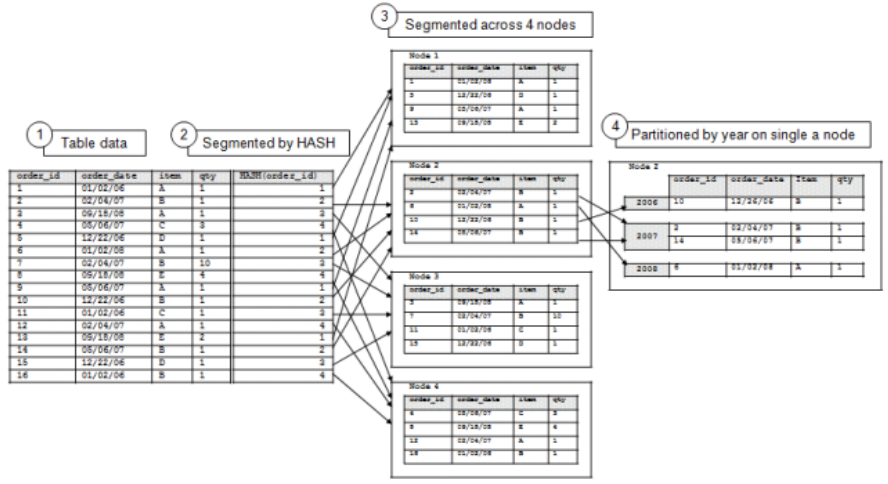
\includegraphics[width=18cm, keepaspectratio]{assets/segm.png}
	\caption{Сегментирование и партиционирование вместе} 
\end{figure}



\subsection{План запроса. Этапы выполнения запроса}

Пусть $X$ --- случайная величина.
